\documentclass[aspectratio=169]{beamer}

% -------------------- Packages --------------------
\usepackage{amsmath, amssymb}
\usepackage{booktabs}
% NOTE: algorithm/algpseudocode often misbehave in Beamer (alignment/spacing).
% We keep them loaded in case you want backup slides, but we do NOT use them in main slides.
\usepackage{algorithm}
\usepackage{algpseudocode}
\usepackage{graphicx}
\usepackage{xcolor}
\usepackage{hyperref}

% -------------------- Theme --------------------
\usetheme{Madrid}
\usecolortheme{default}
\setbeamertemplate{navigation symbols}{}

% -------------------- Metadata --------------------
\title[HPC Polygon Packing via SA]{HPC Simulated Annealing for Non-Convex Polygon Packing in a Square}
\subtitle{Bracketing, Bisection Refinement, Time-Limited Shrink Polish, and Sweep Diagnostics}
\author{Joel Amir D. Maldonado T\"anori}
\institute{Applied Mathematics PhD, University of Arizona}
\date{\today}

% -------------------- Macros --------------------
\newcommand{\R}{\mathbb{R}}
\newcommand{\bb}{\mathbf}
\newcommand{\E}{\mathcal{E}}
\newcommand{\feas}{\mathrm{feas}}
\newcommand{\ov}{\mathrm{ov}}
\newcommand{\out}{\mathrm{out}}
\newcommand{\area}{\mathrm{area}}

\begin{document}

% -------------------- Title --------------------
\begin{frame}
  \titlepage
\end{frame}

% -------------------- NEW: Shape slide right after title --------------------
\begin{frame}{The Shape We Pack}
\centering
% Prefer PDF for best typography; SVG also works in some toolchains.
% Convert: inkscape run/HPC_DEMO/img/N1_job12345_task1_best_N001.svg --export-type=pdf -o run/HPC_DEMO/img/N1_job12345_task1_best_N001.pdf
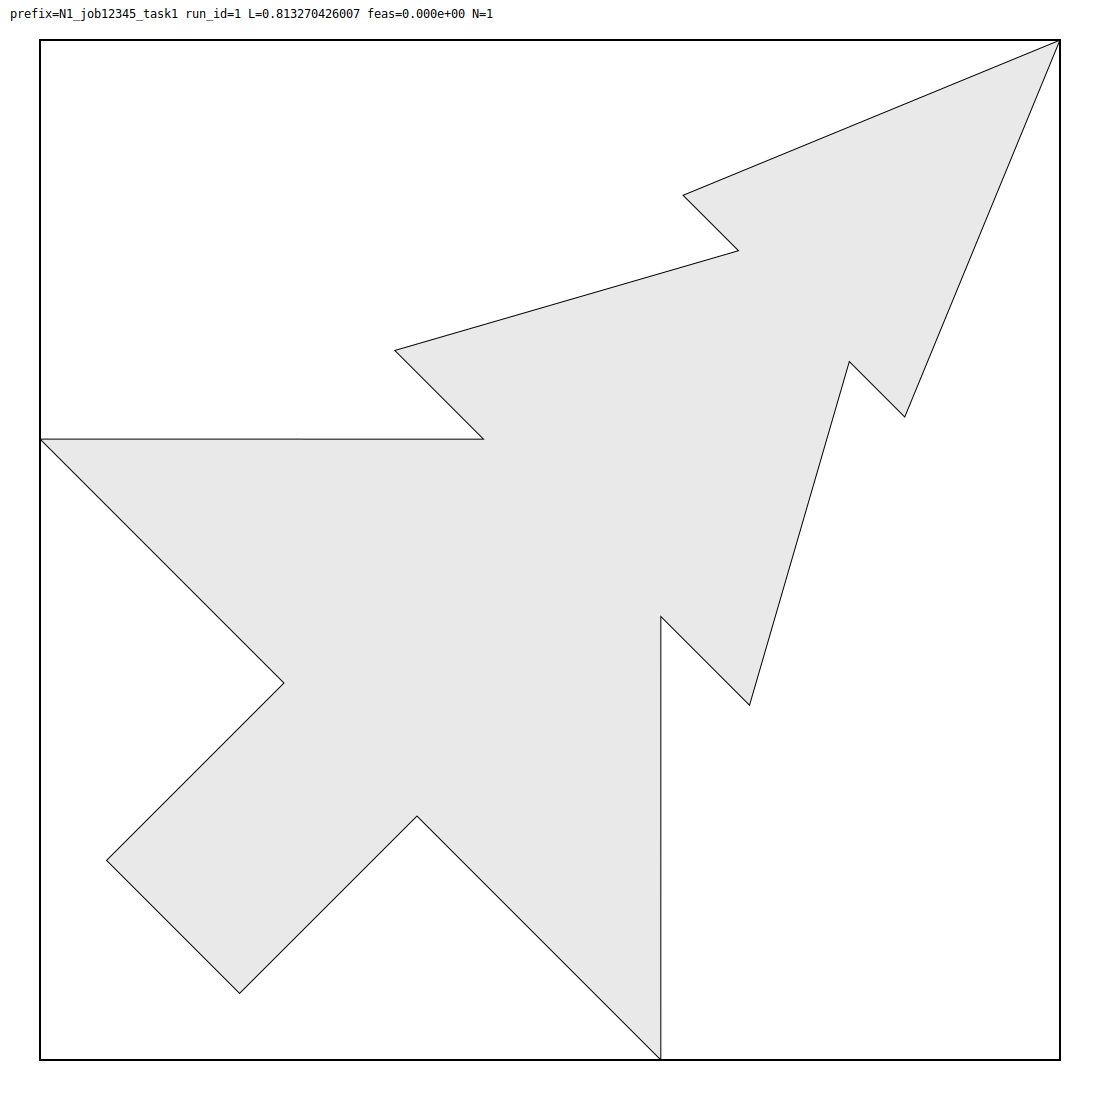
\includegraphics[width=0.55\linewidth]{run/HPC_DEMO/img/N1_job12345_task1_best_N001.pdf}

\medskip
\begin{itemize}
  \item Fixed, non-convex polygon (“tree”)
  \item Identical copies with translation and rotation
  \item Objective: smallest square side length $L$ with no overlap and full containment
\end{itemize}
\end{frame}

% -------------------- Agenda --------------------
\begin{frame}{Agenda}
\begin{enumerate}
  \item Problem and constraints
  \item Geometry model: triangulation + SAT + broad-phase rejects
  \item Energy function, feasibility, and SA moves
  \item Outer optimizer: bracketing + bisection
  \item Time-limited polish: adaptive shrink search + checkpoints
  \item HPC reliability: determinism, file safety, GLIBC considerations
  \item Sweep diagnostics: density, boundary effects, disorder statistics
  \item Best-solution visuals
\end{enumerate}
\end{frame}

% =========================================================
\section{Problem}
% =========================================================

\begin{frame}{Problem Statement}
\textbf{Goal.} Pack $N$ identical copies of a fixed \textbf{non-convex} polygon $P \subset \R^2$ into a square of side length $L$.

\medskip
\textbf{Decision variables (per instance $i=1,\dots,N$):}
\[
(\,c_x^{(i)},\, c_y^{(i)},\, \theta^{(i)}\,) \in \R^2 \times [0,2\pi)
\]
where $(c_x^{(i)},c_y^{(i)})$ is translation and $\theta^{(i)}$ is rotation.

\medskip
\textbf{Constraints.}
\begin{itemize}
  \item \textbf{Non-overlap:} interiors of instances are disjoint.
  \item \textbf{Containment:} each polygon lies inside the square $[-L/2,L/2]^2$.
\end{itemize}

\medskip
\textbf{Objective.} Minimize $L$ (tightest feasible packing).
\end{frame}

\begin{frame}{A Provable Lower Bound (Area Bound)}
Let $\area(P)$ be the polygon area. Then any feasible packing must satisfy:
\[
L^2 \;\ge\; N \cdot \area(P)
\quad\Rightarrow\quad
L \;\ge\; \sqrt{N\,\area(P)}.
\]

\medskip
In code, we keep a strictly provably infeasible threshold:
\[
L_{\text{area}} = \sqrt{N\,\area(P)},\qquad
L_{\text{area-infeas}} = (1-\varepsilon)\,L_{\text{area}}.
\]

\medskip
\textbf{Interpretation.} If $L \le L_{\text{area-infeas}}$, the instance is \textbf{provably infeasible} (no need to run SA).
\end{frame}

% =========================================================
\section{Geometry Model}
% =========================================================

\begin{frame}{Geometry Model: Triangulation + SAT}
We represent the non-convex polygon $P$ by:
\begin{itemize}
  \item A fixed vertex list $\{v_k\}_{k=1}^{N_V}$ in local coordinates.
  \item A fixed triangulation $\{\Delta_t\}_{t=1}^{N_T}$, each triangle uses indices into the vertex list.
\end{itemize}

\medskip
Each instance $i$ produces world vertices:
\[
w_k^{(i)} = R(\theta^{(i)})\,v_k + \begin{bmatrix} c_x^{(i)} \\ c_y^{(i)} \end{bmatrix}.
\]

\medskip
\textbf{Collision test between instances $(i,j)$:}
\begin{enumerate}
  \item Broad-phase AABB overlap
  \item Broad-phase bounding-circle reject
  \item Narrow-phase triangle-triangle SAT for all $(t_a,t_b)$
\end{enumerate}
\end{frame}

\begin{frame}{Broad-Phase Acceleration}
\textbf{AABB reject.} If axis-aligned bounding boxes do not overlap, polygons cannot overlap.

\medskip
\textbf{Bounding-circle reject.} Precompute base radius $r$:
\[
r = \max_k \|v_k\|_2.
\]
If centers are far:
\[
\|c^{(i)}-c^{(j)}\|_2 > 2r
\quad\Rightarrow\quad
\text{no overlap}.
\]

\medskip
\textbf{Uniform grid (spatial hashing).} Each instance belongs to one grid cell; collision checks only consider neighbor cells within a radius based on $2r$.

\medskip
\textbf{Outcome.} Pairwise overlap checks scale with \textit{local neighborhood} interactions rather than $O(N^2)$ in practice.
\end{frame}

\begin{frame}{Containment Penalty via AABB}
Containment is enforced through an \textbf{outside penalty} computed from AABB vs. square:
\[
\out_i(L) = \sum_{\text{violations}} d^2
\]
where $d$ is how far the AABB exceeds $\pm L/2$ in any direction.

\medskip
\textbf{Benefit.} Cheap to compute, robust, and effective when combined with increased penalty weights in Phase B.
\end{frame}

% =========================================================
\section{Energy and Feasibility}
% =========================================================

\begin{frame}{Energy Function and Feasibility Metric}
We separate \textbf{energy} (for SA acceptance) from \textbf{feasibility} (for outer logic).

\medskip
\textbf{Totals:}
\[
\ov(L) = \sum_{i<j} \mathrm{overlap\_penalty}(i,j),\qquad
\out(L) = \sum_{i} \mathrm{outside\_penalty}(i).
\]

\medskip
\textbf{Energy (SA at fixed $L$):}
\[
\E = \lambda\,\ov + \mu\,\out
\]
(with weights scheduled by phase).

\medskip
\textbf{Feasibility metric:}
\[
\feas = \ov + \out.
\]
We declare ``feasible'' if $\feas \le \tau$ for a small tolerance $\tau$ and $L$ is not area-provably infeasible.
\end{frame}

\begin{frame}{Move Set and Incremental Updates}
Each SA iteration chooses a random index $k$ and applies one of:
\begin{itemize}
  \item \textbf{Reinsert (small probability):} randomize $(c_x,c_y,\theta)$ uniformly.
  \item \textbf{Local jitter:} $(c_x,c_y) \leftarrow (c_x,c_y) + \Delta$, $\Delta \sim \mathrm{Unif}([-s,s]^2)$.
  \item \textbf{Rotation mix:} with probability $p_{\text{rot}}$, $\theta \leftarrow \theta + \Delta\theta$.
\end{itemize}

\medskip
\textbf{Incremental bookkeeping.} Only terms involving instance $k$ are recomputed:
\[
\ov \leftarrow \ov + (\ov_k^{\text{new}} - \ov_k^{\text{old}}),\qquad
\out \leftarrow \out + (\out_k^{\text{new}} - \out_k^{\text{old}}).
\]

\medskip
\textbf{Outcome.} Fast inner loop; suitable for HPC sweeps over many $N$.
\end{frame}

% =========================================================
\section{Simulated Annealing (Two-Phase)}
% =========================================================

\begin{frame}{Two-Phase SA Schedule}
We use two sequential phases at fixed $L$:

\medskip
\textbf{Phase A (Explore).}
\begin{itemize}
  \item Higher temperature $T_{\text{start}}\to T_{\text{end}}$
  \item Larger step sizes
  \item Moderate penalties $(\lambda,\mu)$
  \item Purpose: escape poor initializations and reduce gross overlaps/outside
\end{itemize}

\medskip
\textbf{Phase B (Enforce).}
\begin{itemize}
  \item Lower temperatures
  \item Smaller step sizes
  \item \textbf{Penalty ramp:} $(\lambda,\mu) \leftarrow \min((\lambda,\mu)\cdot \rho,\ (\lambda_{\max},\mu_{\max}))$
  \item Purpose: aggressively drive $\feas \to 0$
\end{itemize}
\end{frame}

\begin{frame}{SA Acceptance Rule}
Given current energy $\E$ and proposed energy $\E'$, accept with:
\[
\Delta\E = \E' - \E,
\qquad
\mathbb{P}(\text{accept}) =
\begin{cases}
1, & \Delta\E \le 0,\\
\exp(-\Delta\E / T), & \Delta\E > 0.
\end{cases}
\]

\medskip
We track the best feasibility configuration during the run:
\[
\feas_{\min} = \min_t \feas(t),
\]
and restore to that best configuration at the end of each trial.
\end{frame}

% -------------------- REPLACED: Pseudocode slide (clean, aligned) --------------------
\begin{frame}{Simulated Annealing at Fixed $L$ (Clean Skeleton)}
\begin{block}{State}
\[
x = \{(c_x^{(i)}, c_y^{(i)}, \theta^{(i)})\}_{i=1}^N
\]
\end{block}

\begin{block}{Energy and Feasibility}
\[
\E(x;L) = \lambda\,\ov(x) + \mu\,\out(x;L),
\qquad
\feas(x;L) = \ov(x) + \out(x;L)
\]
\end{block}

\begin{block}{Algorithm Skeleton}
\begin{enumerate}
  \item Initialize $x$ (grid init or warm-start)
  \item Phase A (explore): larger moves, higher temperature
  \item Phase B (enforce): smaller moves, ramp penalties
  \item Track best snapshot (minimum $\feas$) and return it
\end{enumerate}
\end{block}
\end{frame}

% =========================================================
\section{Outer Optimization: Bracket + Bisection}
% =========================================================

\begin{frame}{Outer Loop Overview}
We minimize $L$ via:
\begin{enumerate}
  \item \textbf{Initialize} $L$ from a grid layout (near-square arrangement).
  \item \textbf{Bracketing:} shrink until infeasible (or grow until feasible) to find $[L_{\text{low}},L_{\text{high}}]$.
  \item \textbf{Bisection:} refine the bracket to a tight feasible $L$.
  \item \textbf{Polish:} time-limited stochastic descent to shrink further.
\end{enumerate}

\medskip
\textbf{Reliability constraints.} The area bound prevents invalid brackets; best configurations are carried across $L$ updates by scaling warm-starts.
\end{frame}

\begin{frame}{Bisection Refinement}
Given $L_{\text{low}} < L_{\text{high}}$:
\[
L_{\text{mid}} = \tfrac{1}{2}(L_{\text{low}} + L_{\text{high}}).
\]

\medskip
\textbf{If $L_{\text{mid}} \le L_{\text{area-infeas}}$:} mark infeasible without SA.

\medskip
\textbf{Else:}
\begin{itemize}
  \item Warm-start by scaling best-feasible configuration from $L_{\text{high}}$ to $L_{\text{mid}}$.
  \item Run bounded SA trials at $L_{\text{mid}}$.
  \item If feasible: $L_{\text{high}} \leftarrow L_{\text{mid}}$; else $L_{\text{low}} \leftarrow L_{\text{mid}}$.
\end{itemize}

\medskip
After $k$ steps, bracket width shrinks by $2^{-k}$.
\end{frame}

% =========================================================
\section{Polish: Time-Limited Shrink Search}
% =========================================================

\begin{frame}{Polish Stage: Adaptive Shrink Search}
After bisection, we have a strong feasible configuration at $L^\star$.

\medskip
\textbf{Attempt a shrink:}
\[
L_{\text{try}} = L^\star (1-\epsilon)
\]
Scale positions, then run a few SA trials.

\medskip
\textbf{Adaptive control.} Tune $\epsilon$ based on recent success rate (stochastic descent with backoff) until time limit is reached.
\end{frame}

\begin{frame}{Time Limit, Checkpoints, and SIGTERM}
\textbf{Time-limited polish.} We cap polish runtime (e.g., 900s) to guarantee completion in Slurm arrays.

\medskip
\textbf{Periodic checkpoints (every $\Delta t$ seconds):}
\begin{itemize}
  \item \texttt{csv/<prefix>\_checkpoint\_Nxxx.csv}
  \item \texttt{img/<prefix>\_checkpoint\_Nxxx.svg}
\end{itemize}

\medskip
\textbf{SIGTERM handling.} Near walltime Slurm sends SIGTERM; the handler:
\begin{itemize}
  \item flushes \textbf{best snapshot} to best and checkpoint files,
  \item exits cleanly.
\end{itemize}

\medskip
\textbf{Outcome.} Even canceled jobs produce usable artifacts.
\end{frame}

% =========================================================
\section{HPC Engineering}
% =========================================================

\begin{frame}{HPC Engineering: Determinism and File Safety}
\textbf{Deterministic seeds.} Each trial seed is derived from:
\[
\text{seed} = f(\text{base\_seed},\ \text{run\_id},\ \text{trial\_id})
\]
(e.g., SplitMix64 diffusion) for reproducibility across array jobs.

\medskip
\textbf{Unique output prefixes.}
\[
\texttt{out\_prefix} = \texttt{N\{N\}\_job\{job\}\_task\{task\}}
\]
prevents file collisions under concurrency.

\medskip
\textbf{Build environment.} Compile on compute nodes (or use cluster toolchain) to avoid GLIBC mismatch between login/desktop and compute nodes.
\end{frame}

\begin{frame}{Complexity Notes and Practical Performance}
\textbf{Worst case.} Collision evaluation can be heavy, but practice is improved by:
\begin{itemize}
  \item grid neighbor enumeration (local pairs),
  \item AABB + bounding-circle rejects (broad phase),
  \item small fixed triangulation size ($N_T$ constant),
  \item incremental updates per move (only one instance changes).
\end{itemize}

\medskip
\textbf{Scaling expectation.} Runtime grows with local density and neighbor interactions, typically milder than $O(N^2)$.
\end{frame}

% -------------------- NEW: Natural language sweep summary slide --------------------
\begin{frame}{Overnight HPC Sweep: Execution Summary}
\begin{block}{What Was Run}
A Slurm job array solved \textbf{200 independent packing problems}, one per
$N=1,\dots,200$, using identical solver logic and fixed per-task budgets.
\end{block}

\begin{block}{Resource Budget}
\begin{itemize}
  \item Up to \textbf{20 tasks in parallel} (\texttt{\#SBATCH --array=1-200\%20})
  \item \textbf{30 minutes wall time per task} (\texttt{\#SBATCH --time=00:30:00})
  \item 1 CPU core, 2 GB memory per task
\end{itemize}
\end{block}

\begin{block}{Time Allocation Within Each Task}
\begin{itemize}
  \item \textbf{Bracketing + bisection:} bounded SA trials (designed to always finish)
  \item \textbf{Polish stage:} time-limited to \textbf{12 minutes}
  \item \textbf{Checkpoints:} every 3 minutes during polish
  \item \textbf{Termination safety:} SIGTERM handler flushes best artifacts before exit
\end{itemize}
\end{block}
\end{frame}

% -------------------- NEW: Parallelization model slide --------------------
\begin{frame}{Parallelization Model}
\begin{block}{Type of Parallelism}
\textbf{Embarrassingly parallel parameter sweep.}
Each value of $N$ is solved independently:
\[
\text{Task } N \quad\longleftrightarrow\quad \text{one SLURM array element}.
\]
\end{block}

\begin{block}{Why This Scales Well}
\begin{itemize}
  \item No inter-task communication or synchronization
  \item No MPI overhead; pure throughput scaling
  \item Fault isolation: failure at one $N$ does not affect others
\end{itemize}
\end{block}

\begin{block}{Scheduling Benefits}
\begin{itemize}
  \item Slurm load-balances variable runtimes across $N$
  \item Concurrency cap prevents queue flooding
  \item Natural extension to longer per-$N$ runs or replicated runs per $N$
\end{itemize}
\end{block}
\end{frame}

% -------------------- NEW: Reproducibility slide --------------------
\begin{frame}{Reproducibility Under Parallel Execution}
\begin{block}{Deterministic Seeding}
Each task uses a fixed base seed combined with:
\[
\text{seed} = f(\text{base seed},\; N,\; \text{trial id}),
\]
ensuring reproducibility regardless of execution order or node placement.
\end{block}

\begin{block}{File Safety}
\begin{itemize}
  \item Unique output prefixes: \texttt{N\{N\}\_job\{job\}\_task\{task\}}
  \item No collisions under concurrent tasks
  \item Safe output on shared filesystems
\end{itemize}
\end{block}

\begin{block}{Reliability}
\begin{itemize}
  \item SIGTERM delivered before wall time (buffer) to flush artifacts
  \item Periodic checkpoints reduce risk of losing progress
\end{itemize}
\end{block}
\end{frame}

% =========================================================
\section{Sweep Diagnostics}
% =========================================================

\begin{frame}{Sweep Outputs and Aggregation}
For each $N$, the code writes:
\begin{itemize}
  \item \texttt{img/<prefix>\_best\_Nxxx.svg} and \texttt{csv/<prefix>\_best\_polys\_Nxxx.csv}
  \item \texttt{img/<prefix>\_checkpoint\_Nxxx.svg} and \texttt{csv/<prefix>\_checkpoint\_Nxxx.csv}
\end{itemize}

\medskip
A sweep analysis script aggregates all best CSVs into:
\begin{itemize}
  \item \texttt{analysis/summary.csv} (one row per $N$)
  \item \texttt{analysis/plots/*.png} (diagnostic graphs)
\end{itemize}

\medskip
These plots quantify \textbf{how tight} the packing is and \textbf{why} larger $N$ can become loose.
\end{frame}

\begin{frame}{Key Packing Quality Metrics}
Let $\area(P)$ be polygon area and $L(N)$ be best feasible side length for size $N$.

\medskip
\textbf{Density (primary):}
\[
\rho(N) = \frac{N\,\area(P)}{L(N)^2}
\qquad
\text{(higher is better)}
\]

\medskip
\textbf{Empty area (slack):}
\[
\Delta A(N) = L(N)^2 - N\,\area(P)
\]

\medskip
\textbf{Boundary fraction (boundary waste proxy):}
fraction of centers within distance $k r$ of the square boundary, where $r$ is the polygon bounding radius.

\medskip
\textbf{Structure/disorder:}
\begin{itemize}
  \item nearest-neighbor distance statistics (mean / std),
  \item orientation entropy of $\{\theta_i\}$ (high entropy $\Rightarrow$ amorphous).
\end{itemize}
\end{frame}

\begin{frame}{Density vs $N$}
\centering
\includegraphics[width=0.92\linewidth]{../../run/HPC_DEMO/analysis/plots/density_vs_N.png}

\vspace{1mm}
\small
Interpretation: decreasing density at large $N$ suggests boundary waste and/or failure to discover a strong interior motif.
\end{frame}

\begin{frame}{Density vs $1/\sqrt{N}$ (Boundary Scaling Diagnostic)}
\centering
\includegraphics[width=0.92\linewidth]{../../run/HPC_DEMO/analysis/plots/density_vs_inv_sqrtN.png}

\vspace{1mm}
\small
If this plot is approximately linear, the deficit is dominated by boundary effects; curvature indicates deeper structural inefficiency.
\end{frame}

\begin{frame}{Empty Area (Slack) vs $N$}
\centering
\includegraphics[width=0.92\linewidth]{../../run/HPC_DEMO/analysis/plots/area_gap_vs_N.png}

\vspace{1mm}
\small
Large $\Delta A$ at high $N$ is consistent with visible voids around the packing.
\end{frame}

\begin{frame}{Boundary Fraction vs $N$}
\centering
\includegraphics[width=0.92\linewidth]{../../run/HPC_DEMO/analysis/plots/boundary_fraction_vs_N.png}

\vspace{1mm}
\small
High boundary fraction indicates significant mass near the square edges and suggests boundary-limited performance.
\end{frame}

\begin{frame}{Nearest-Neighbor Spacing vs $N$}
\centering
\includegraphics[width=0.92\linewidth]{../../run/HPC_DEMO/analysis/plots/nn_mean_vs_N.png}

\vspace{1mm}
\small
Increasing mean nearest-neighbor distance indicates wasted interior space; high variance suggests disordered configurations.
\end{frame}

\begin{frame}{Orientation Entropy vs $N$}
\centering
\includegraphics[width=0.92\linewidth]{../../run/HPC_DEMO/analysis/plots/orientation_entropy_vs_N.png}

\vspace{1mm}
\small
High entropy suggests an amorphous phase; a collapse toward lower entropy often indicates a repeating local motif (tiling-like structure).
\end{frame}

\begin{frame}{Interpreting the Diagnostics}
\textbf{Case A: boundary-limited (good interior, bad boundary).}
\begin{itemize}
  \item density vs $1/\sqrt{N}$ approximately linear,
  \item interior spacing stable, but boundary fraction high.
\end{itemize}
\textbf{Response:}
warm-start from a periodic tiling; fit near-square patches; boundary-aware refinement.

\medskip
\textbf{Case B: motif failure (interior also loose).}
\begin{itemize}
  \item density flattens too low,
  \item NN mean grows and orientation entropy remains high.
\end{itemize}
\textbf{Response:}
discover small periodic motifs (periodic boundary SA), then tile; add structured moves / templates.
\end{frame}

% =========================================================
\section{Results}
% =========================================================

% -------------------- NEW: Best packings montage slides (requested Ns) --------------------
\begin{frame}{Best Solutions Across $N$ (Small)}
\begin{columns}
\column{0.33\textwidth}
\centering
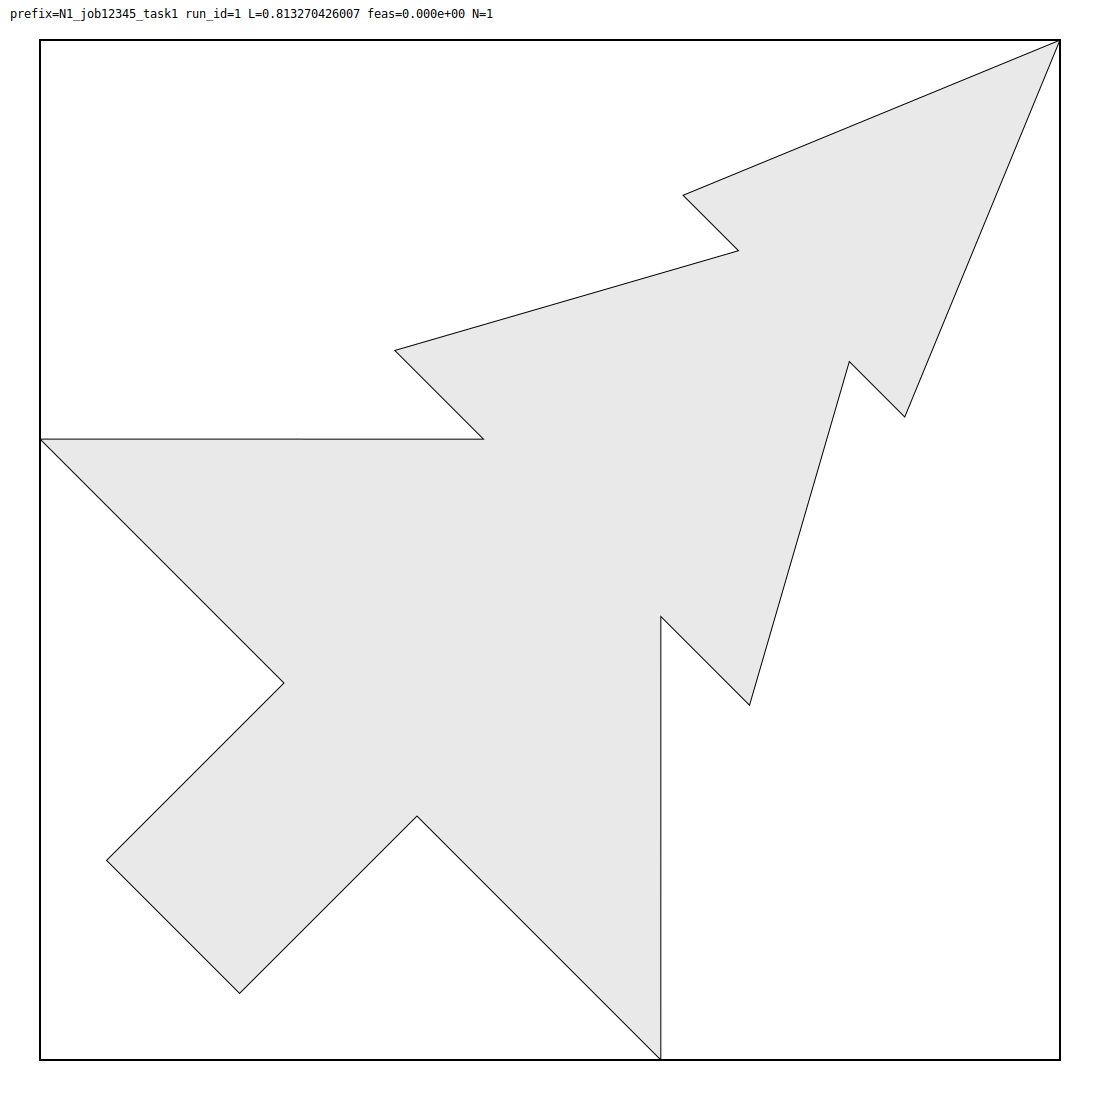
\includegraphics[width=\linewidth]{run/HPC_DEMO/img/N1_job12345_task1_best_N001.pdf}\\
\small $N=1$

\column{0.33\textwidth}
\centering
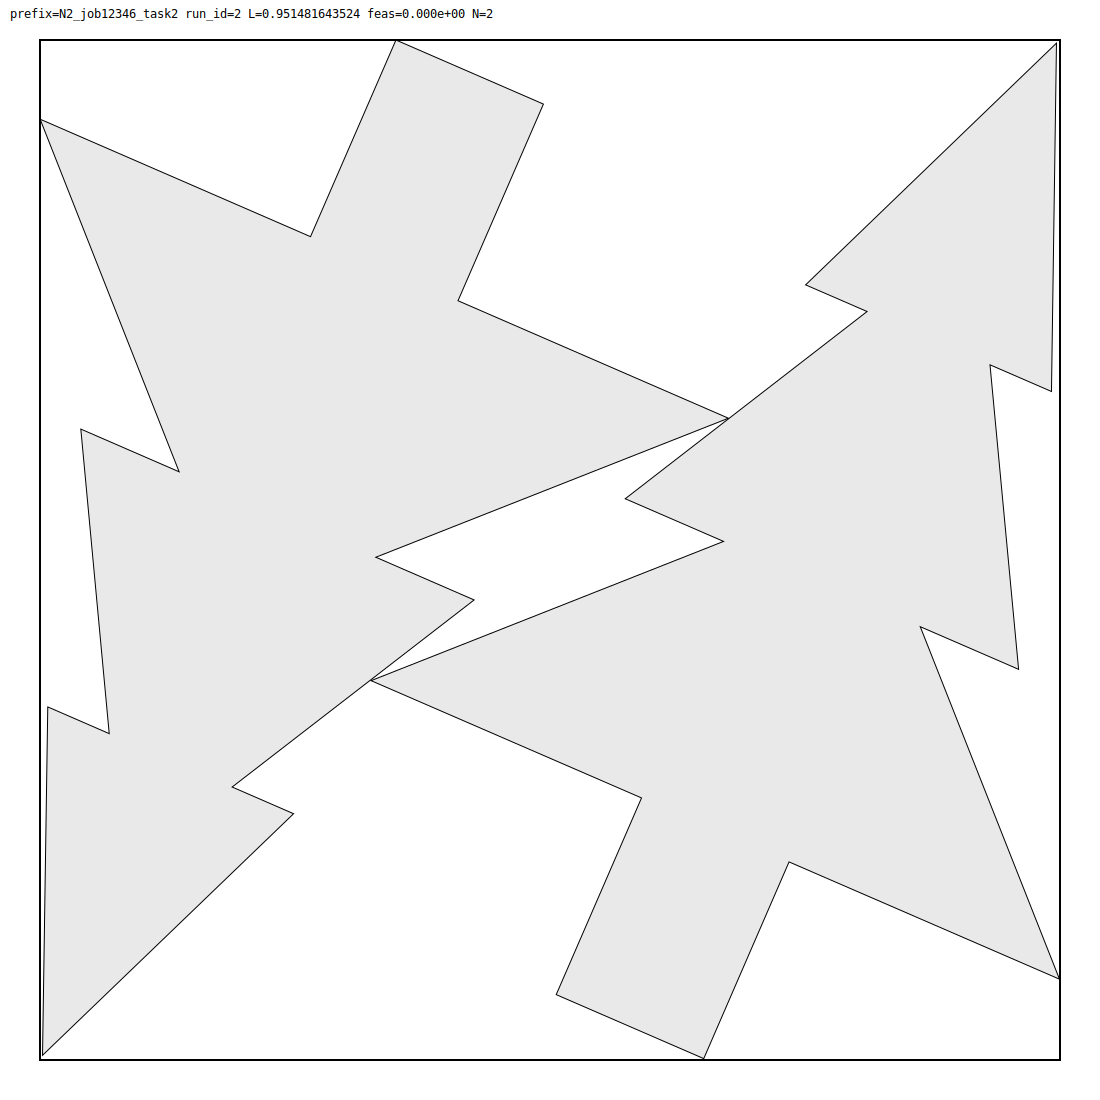
\includegraphics[width=\linewidth]{run/HPC_DEMO/img/N2_job12346_task2_best_N002.pdf}\\
\small $N=2$

\column{0.33\textwidth}
\centering
\includegraphics[width=\linewidth]{run/HPC_DEMO/img/N5_job12346_task5_best_N005.pdf}\\
\small $N=5$
\end{columns}
\end{frame}

\begin{frame}{Best Solutions Across $N$ (Medium)}
\begin{columns}
\column{0.5\textwidth}
\centering
% Replace with your actual path after converting the SVG for N=10
\includegraphics[width=\linewidth]{run/HPC_DEMO/img/N10_jobXXXX_task10_best_N010.pdf}\\
\small $N=10$

\column{0.5\textwidth}
\centering
% Replace with your actual path after converting the SVG for N=20
\includegraphics[width=\linewidth]{run/HPC_DEMO/img/N20_jobXXXX_task20_best_N020.pdf}\\
\small $N=20$
\end{columns}
\end{frame}

\begin{frame}{Best Solutions Across $N$ (Large)}
\begin{columns}
\column{0.5\textwidth}
\centering
% Replace with your actual path after converting the SVG for N=50
\includegraphics[width=\linewidth]{run/HPC_DEMO/img/N50_jobXXXX_task50_best_N050.pdf}\\
\small $N=50$

\column{0.5\textwidth}
\centering
% Replace with your actual path after converting the SVG for N=100
\includegraphics[width=\linewidth]{run/HPC_DEMO/img/N100_jobXXXX_task100_best_N100.pdf}\\
\small $N=100$
\end{columns}
\end{frame}

\begin{frame}{Best Solution at the Largest Studied $N$}
\centering
% Replace with your actual path after converting the SVG for N=200
\includegraphics[width=0.85\linewidth]{run/HPC_DEMO/img/N200_jobXXXX_task200_best_N200.pdf}

\medskip
\begin{itemize}
  \item Visible unused boundary regions at large $N$
  \item Suggests boundary waste and/or failure to discover a global repeating motif
  \item Motivates compactification and tiling-inspired warm-starts
\end{itemize}
\end{frame}

% -------------------- NEW: Observation + next-steps slide --------------------
\begin{frame}{Observations and Next Steps}
\begin{block}{Observed Behavior}
\begin{itemize}
  \item Small $N$: dense, visually near-optimal packings
  \item Large $N$: increasing slack, empty regions near boundary, disordered orientations
\end{itemize}
\end{block}

\begin{block}{Immediate Next Steps}
\begin{itemize}
  \item \textbf{Post-processing (cheap):} greedy projection + shrink loop (boundary tightening)
  \item \textbf{Local refinement:} introduce smooth penalties and apply L-BFGS-B
  \item \textbf{Structure discovery:} periodic-boundary SA to find motifs, then tile into near-square patches
\end{itemize}
\end{block}
\end{frame}

\begin{frame}{Summary}
\begin{itemize}
  \item Non-convex polygon packing solved with \textbf{two-phase SA} + robust geometry checks.
  \item \textbf{Area bound} provides provable infeasibility cutoff.
  \item \textbf{Bracket + bisection} yields a tight feasible $L$ reliably.
  \item \textbf{Time-limited polish} improves $L$ under strict HPC budgets and guarantees artifacts.
  \item Sweep diagnostics quantify \textbf{density}, \textbf{boundary waste}, and \textbf{structural disorder}.
\end{itemize}

\medskip
\textbf{Next steps:}
\begin{itemize}
  \item periodic-boundary runs to estimate infinite-tiling density,
  \item template/warm-start based on discovered motifs,
  \item targeted long-polish on hard $N$ values.
\end{itemize}
\end{frame}

\begin{frame}
\centering
\Large Questions?
\end{frame}

\end{document}
